\vspace{-3mm}
\section{FKM Richtlinien}{}
    \subsection{Auslastungsgrad}
     
        \subsubsection{Definitionen}
            \begin{enumerate}[noitemsep]
                \item $\sigma_{v}$: Vergleichsspannung im Nachweispunkt
                \item $\sigma_{SK}$: Materialfestgkeit, bauteilspezifisch
                \item $J_{ges}$: Sicherheitsfaktor (Gesamtsicherheitsfaktor)
            \end{enumerate}
            \[a_{SK} = \frac{\sigma_{v}}{\sigma_{sk}/J_{ges}} \]
    
        \subsubsection{Mehrachsigkeit}
            Falls $h > 1.33$ zusätzlicher Nachweis erforderlich! 
            \[ h = \frac{\frac{1}{3} \textrm{Spur}[T]}{\sigma_{Mises}} \quad \textrm{[T]: Spannungstensor}\]
        \subsubsection{Bauteilfestigkeit $\sigma_{\textrm{SK}}$}
            An Normprobe gemessene Fliessgrenze erffordert meistens Korrektur! \\$R_P$: Fliessgrenze Bauteil; $R_{P,N}$: Fliessgrenze Normporbe.
            \vspace{-2mm}
            \[R_P = K_{d,P}\cdot K_A\cdot R_{P,N}\]
            \vspace{-5mm}
            \[\sigma_{\textrm{SK}}=R_p\cdot n_{\textrm{pl}} \quad\textrm{mit:}\quad \small n_{\textrm{pl}}=\textrm{min} \left( \sqrt{ \frac{E\cdot\varepsilon_{\textrm{ertr}}}{R_p}};K_p \right) \]\normalsize
            Hom. Spannungsverteilung: $n_{\textrm{pl}}=1$ (Keine Reserve)
            \vspace{-2mm}
            \[K_p: \textrm{platische Formzahl} = \frac{\textrm{vollplastische Traglast}}{\textrm{elastische Grenzlast}}\]
            vollpl.: aus FE; el. Grenzl.: wenn $\sigma_v = R_p$ erreicht.
        \subsubsection{Sicherheitsfaktor $J_{\textrm{ges}}$}
        \small\[J_{\textrm{ges}}= J_s \cdot \left[ J_z \cdot \textrm{max}\left(\frac{J_m \cdot R_p}{R_m}; J_p \right) \right] \]\normalsize
        $J_s$: Lastfaktor (Sicher:=1); $J_z$: Schweissteile; $J_p$: plastifizierung
        \begin{center}
            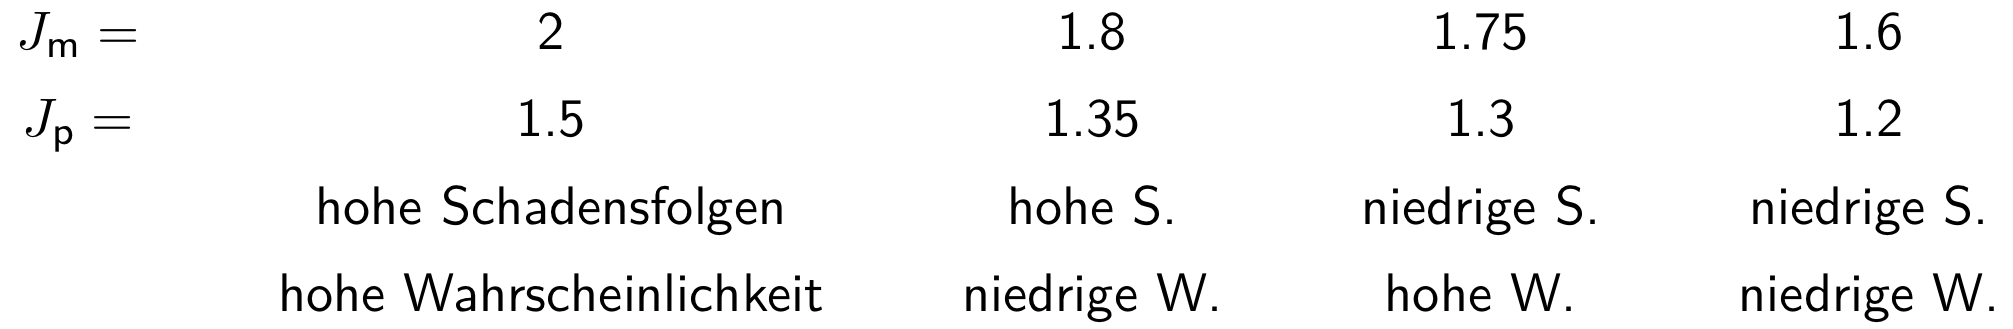
\includegraphics[width=0.8\linewidth]{05/Sicherheitsfaktoren.png}
        \end{center}
    
    \subsection{BSP}
        \subsubsection{Dimensionieren eines Kessels mit Loch nach FKM}
        Ziel: Kessel so dimensioniert, dass keine zusätzlich Verstrebungen am Loch notwendig sind. $\rightarrow$  $ a_{SK}<1 $
        
        Gegeben: $ \sigma_v = 590 \textrm{MPa} $ (aus FE-Analyse); $ \varepsilon_{ertr} $ (Bruchdehnung); $K_A = 1 \textrm{; } K_{d,p} = 0.92 \textrm{; } R_e = 900 \textrm{MPa} $
        
        Vorgehen:
        $ a_{{SK}} = \frac{\frac{\sigma_v}{\sigma_{{SK}}}}{J_{ges}}  \rightarrow  \sigma_v \cdot J_{ges} < \sigma_{{SK}} $
        
        Wegen Mehrachsigkeit, kein weiterer Nachweis nötig
        
        $ h = \frac{\frac{1}{3}(\sigma_1+\sigma_2+\sigma_3)}{\sigma_{{v,Mises}}}=\frac{1}{3} 
        \rightarrow  h_{} < 1.33_{} $
        
        Bauteilspezifische Materialfestigkeit $ \sigma_{SK} $ berechnen:
        
        $ \sigma_{SK} = R_p \cdot n_{pl} $;
        $ R_p = K_{d,p} \cdot K_A \cdot R_e $; %fliessgrenze am Bauteil
        %Kdp technologischer Grössenfaktor  Ka anisotropie
        $ n_{pl} = \textrm{min}(\sqrt{\frac{E \cdot \varepsilon_{ertr}}{R_p}}; K_p) $
        
        Sicherheitsfaktor berechnen
        
        $ J_{ges} = J_s \cdot ( J_z \cdot \textrm{max}(\frac{J_m \cdot R_p}{R_m} ; J_p) $
        
        $ {J_{ges}} \textrm{ und } \sigma_{SK}$ in unserer Ursprünglichen Gleichung eingesetzt ergibt ${a_{SK} = 0.4 < 1} $ $\rightarrow$ FKM erfüllt
